%%%%%%%%%%%%%%%%%%%%%%%%%%%%%%%%%%%%%%%%%
% Jacobs Landscape Poster
% LaTeX Template
% Version 1.1 (14/06/14)
%
% Created by:
% Computational Physics and Biophysics Group, Jacobs University
% https://teamwork.jacobs-university.de:8443/confluence/display/CoPandBiG/LaTeX+Poster
% 
% Further modified by:
% Nathaniel Johnston (nathaniel@njohnston.ca)
%
% This template has been downloaded from:
% http://www.LaTeXTemplates.com
%
% License:
% CC BY-NC-SA 3.0 (http://creativecommons.org/licenses/by-nc-sa/3.0/)
%
%%%%%%%%%%%%%%%%%%%%%%%%%%%%%%%%%%%%%%%%%

%----------------------------------------------------------------------------------------
%	PACKAGES AND OTHER DOCUMENT CONFIGURATIONS
%----------------------------------------------------------------------------------------

\documentclass[final]{beamer}

\usepackage[scale=1.24]{beamerposter} % Use the beamerposter package for laying out the poster
\usepackage[utf8]{inputenc}
\usepackage[spanish]{babel}	
\usepackage{caption}
\usepackage{subcaption} 

\usetheme{confposter} % Use the confposter theme supplied with this template

\setbeamercolor{block title}{fg=ngreen,bg=white} % Colors of the block titles
\setbeamercolor{block body}{fg=black,bg=white} % Colors of the body of blocks
\setbeamercolor{block alerted title}{fg=white,bg=dblue!70} % Colors of the highlighted block titles
\setbeamercolor{block alerted body}{fg=black,bg=dblue!10} % Colors of the body of highlighted blocks
% Many more colors are available for use in beamerthemeconfposter.sty

%-----------------------------------------------------------
% Define the column widths and overall poster size
% To set effective sepwid, onecolwid and twocolwid values, first choose how many columns you want and how much separation you want between columns
% In this template, the separation width chosen is 0.024 of the paper width and a 4-column layout
% onecolwid should therefore be (1-(# of columns+1)*sepwid)/# of columns e.g. (1-(4+1)*0.024)/4 = 0.22
% Set twocolwid to be (2*onecolwid)+sepwid = 0.464
% Set threecolwid to be (3*onecolwid)+2*sepwid = 0.708

\newlength{\sepwid}
\newlength{\onecolwid}
\newlength{\twocolwid}
\newlength{\threecolwid}
\setlength{\paperwidth}{48in} % A0 width: 46.8in
\setlength{\paperheight}{36in} % A0 height: 33.1in
\setlength{\sepwid}{0.024\paperwidth} % Separation width (white space) between columns
\setlength{\onecolwid}{0.22\paperwidth} % Width of one column
\setlength{\twocolwid}{0.464\paperwidth} % Width of two columns
\setlength{\threecolwid}{0.708\paperwidth} % Width of three columns
\setlength{\topmargin}{-0.5in} % Reduce the top margin size
%-----------------------------------------------------------

\usepackage{graphicx}  % Required for including images

\usepackage{booktabs} % Top and bottom rules for tables

%----------------------------------------------------------------------------------------
%	TITLE SECTION 
%----------------------------------------------------------------------------------------

\title{Autómata celular para la caracterización del tráfico} % Poster title

\author{Alejandro Aguilar-Salas, Carlos Manuel Rodríguez-Martínez} % Author(s)

\institute{Departamento de Física, Universidad Veracruzana} % Institution(s)

%----------------------------------------------------------------------------------------

\begin{document}

\addtobeamertemplate{block end}{}{\vspace*{2ex}} % White space under blocks
\addtobeamertemplate{block alerted end}{}{\vspace*{2ex}} % White space under highlighted (alert) blocks

\setlength{\belowcaptionskip}{2ex} % White space under figures
\setlength\belowdisplayshortskip{2ex} % White space under equations

\begin{frame}[t] % The whole poster is enclosed in one beamer frame

\begin{columns}[t] % The whole poster consists of three major columns, the second of which is split into two columns twice - the [t] option aligns each column's content to the top

\begin{column}{\sepwid}\end{column} % Empty spacer column

\begin{column}{\onecolwid} % The first column

%----------------------------------------------------------------------------------------
%	OBJECTIVES
%----------------------------------------------------------------------------------------

\begin{alertblock}{Objetivos}

Observar el efecto que causan en el tráfico los elementos viales como:
\begin{itemize}
\item Semáforos
\item Cruces
\item Topes
\item Múltiples carriles
\end{itemize}
en una simulación del tráfico basada en un autómata celular.

\end{alertblock}

%----------------------------------------------------------------------------------------
%	INTRODUCTION
%----------------------------------------------------------------------------------------

\begin{block}{Introducción}

En este trabajo presentamos una simulación computacional
de un modelo de trafico vehicular con autómatas celulares. Nuestra 
simulación está basada en el modelo de Nagel y Schreckenberg, y 
hemos incluido la posibilidad de tener varios carriles, automóviles autónomos,
como se espera tener en un futuro próximo, así como la existencia
de "topes" (algo poco estudiado ya que es una medida de control que
existe en muy pocos países) y la posibilidad de tener intersecciones
el en camino.

\end{block}

%------------------------------------------------

\begin{figure}
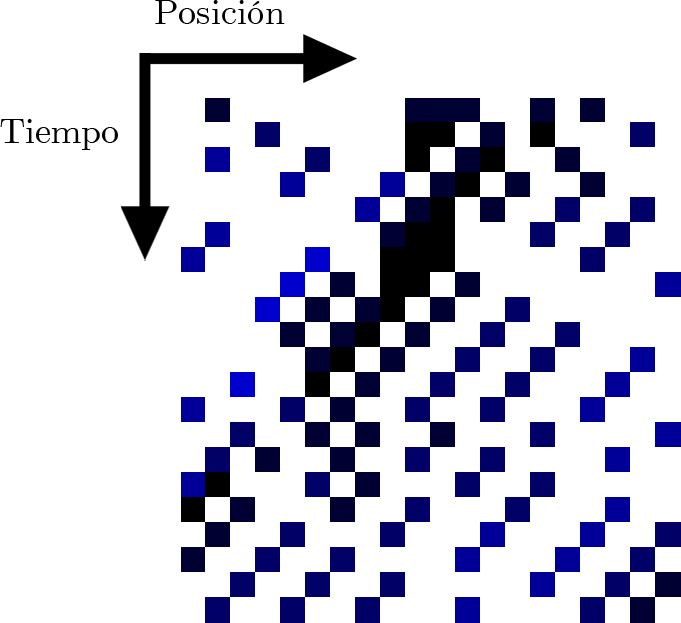
\includegraphics[width=0.8\linewidth]{img/ca_flechas}
\caption{Representación de autómata celular de tamaño $20$ y evolucionado con $20$ iteraciones. En azul los vehículos con mayor velocidad.}
\end{figure}

%----------------------------------------------------------------------------------------

\end{column} % End of the first column

\begin{column}{\sepwid}\end{column} % Empty spacer column

\begin{column}{\twocolwid} % Begin a column which is two columns wide (column 2)

\begin{columns}[t,totalwidth=\twocolwid] % Split up the two columns wide column

\begin{column}{\onecolwid}\vspace{-.6in} % The first column within column 2 (column 2.1)

%----------------------------------------------------------------------------------------
%	MATERIALS
%----------------------------------------------------------------------------------------

\begin{block}{Modelo de tráfico}

Se elabora un arreglo unidimensional de longitud $S$. Cada vehículo tiene una velocidad entera que se encuentra entre $[0,v_{max}]$. La regla de evolución es
\begin{enumerate}

\item \textbf{Aceleración}: Si la velocidad $v$ de un vehículo es menor que $v_{max}$ y la distancia con el siguiente auto es mayor que $v+1$, la velocidad se aumenta en una unidad $(v \to v+1)$.

\item \textbf{Frenado} (debido a los demás autos): Si un vehículo en la posición $i$ observa al siguiente vehículo en la posición $i+j$, reduce su velocidad a $j-1$ $(v\to j-1)$.

\item \textbf{Aleatorización}: Con probabilidad $p$, la velocidad de cada vehículo (si es mayor que cero) disminuye en uno $(v\to v-1)$.

\item \textbf{Movimiento vehicular}: Cada vehículo avanza $v$ espacios.

\end{enumerate}

\end{block}

\begin{block}{Mediciones}

Medimos el flujo de autos como
\[
	q = \frac{1}{T} \sum_{t = t_0+1}^{t_0 + T} n_{i,i+1} (t),
\]
donde $n_{i,i+1} (t) = 1$ si se detecta que un auto pasa por esa casilla.

\end{block}

\begin{block}{Semáforos}

Se añade la posición del semáforo a la regla de frenado. Tienen tiempo de cerrado y de apertura.

\begin{figure}[h!]
\begin{subfigure}{.5\textwidth}
	\centering
	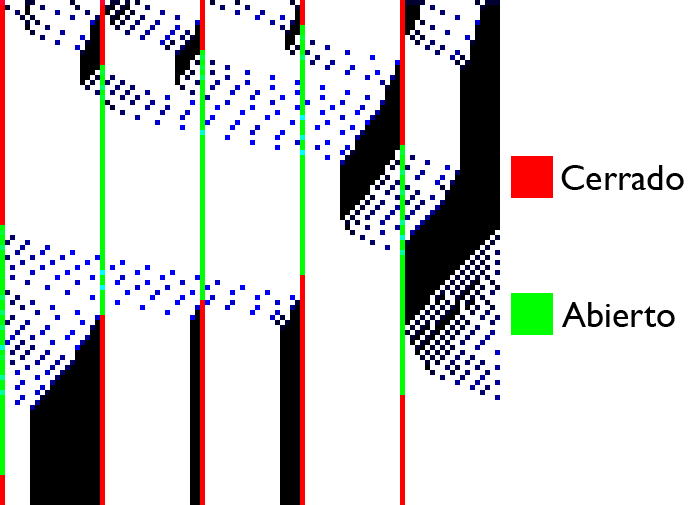
\includegraphics[scale=0.4]{img/semaforo_ac}
	\caption{Representación del AC.}
\end{subfigure}%
\begin{subfigure}{.5\textwidth}
	\centering
	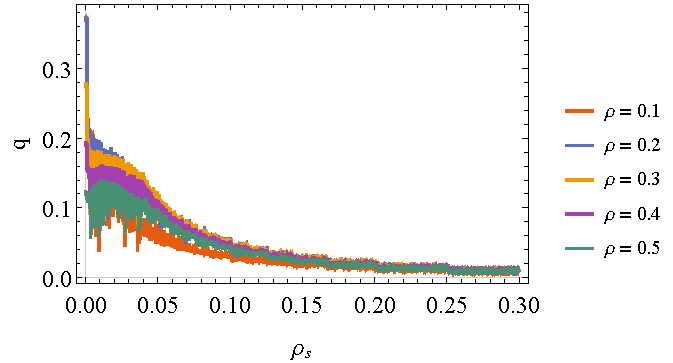
\includegraphics[scale=1.2]{img/flow_vs_semaphore_density}
	\caption{Flujo respecto a densidad de semáforos.}
\end{subfigure}%
\end{figure}

\end{block}

%----------------------------------------------------------------------------------------

\end{column} % End of column 2.1

\begin{column}{\onecolwid}\vspace{-.6in} % The second column within column 2 (column 2.2)

%----------------------------------------------------------------------------------------
%	METHODS
%----------------------------------------------------------------------------------------

\begin{block}{Vehículos autónomos}

Los vehículos autónomos no sufren aleatorización y tienen tiempo de reacción instantáneo.

\begin{figure}[h!]
\begin{subfigure}{.5\textwidth}
	\centering
	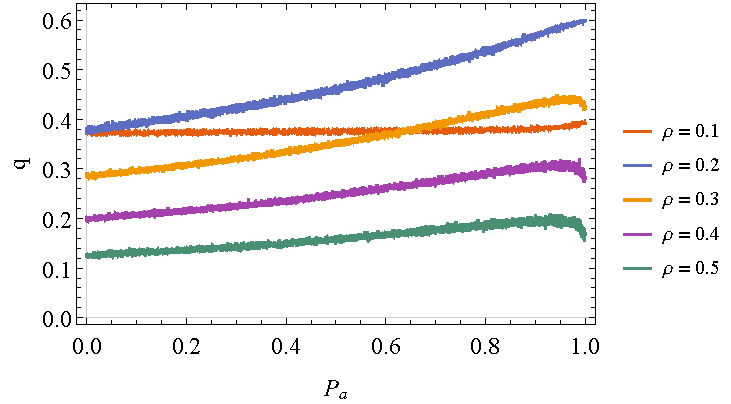
\includegraphics[scale=1.1]{img/flow_vs_aut_cars}
	\caption{Flujo respecto a porcentaje de vehículos autónomos.}
\end{subfigure}%
\begin{subfigure}{.5\textwidth}
	\centering
	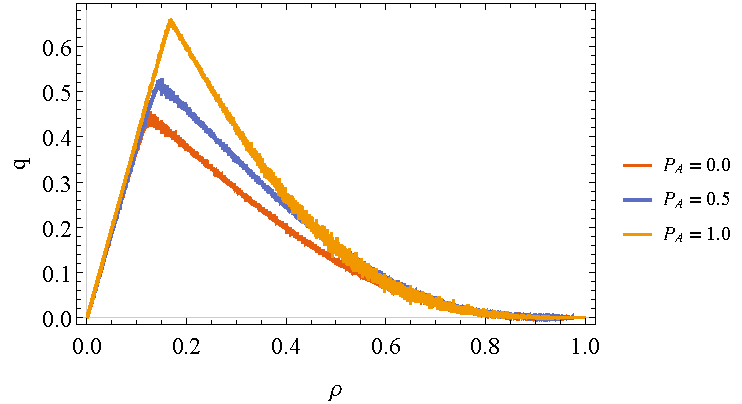
\includegraphics[scale=1.1]{img/flow_vs_density_aut}
	\caption{Flujo respecto a densidad.}
\end{subfigure}%
\end{figure}

\end{block}

\begin{block}{Topes}
Si un vehículo con $v > 1$ en la posición $i$ observa un tope en la posición $i+j$, y $j < c \, v_{max}$ reduce su velocidad en una unidad.

\begin{figure}[h!]
\begin{subfigure}{.5\textwidth}
	\centering
	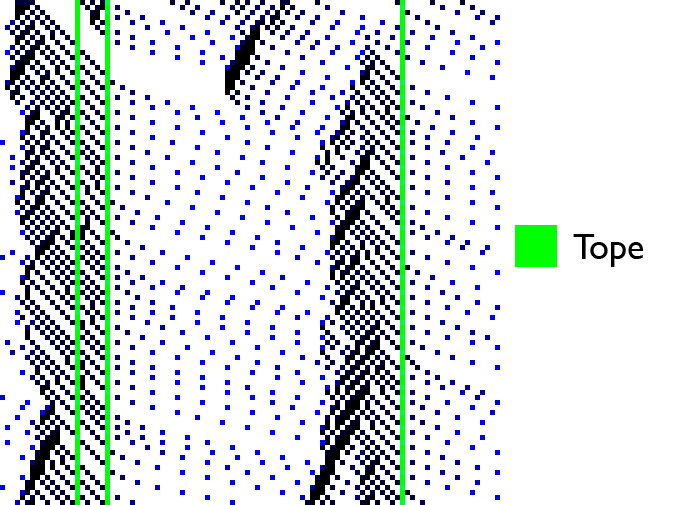
\includegraphics[scale=0.4]{img/tope_ac}
	\caption{Flujo respecto a porcentaje de vehículos autónomos.}
\end{subfigure}%
\begin{subfigure}{.5\textwidth}
	\centering
	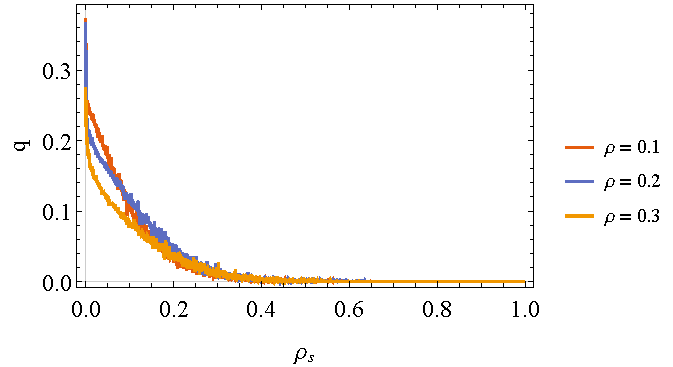
\includegraphics[scale=1.2]{img/flow_vs_stop_density}
	\caption{Flujo respecto a densidad.}
\end{subfigure}%
\end{figure}

\end{block}

\begin{block}{Múltiples carriles}
Para extender el modelo a múltiples carriles se añade un paso extra. En este se verifica si el vehículo no puede acelerar, entonces busca si en los adyacentes puede acelerar sin afectar el tráfico. Si dos carriles fueron marcados como disponibles, selecciona el de la izquierda.

\begin{figure}
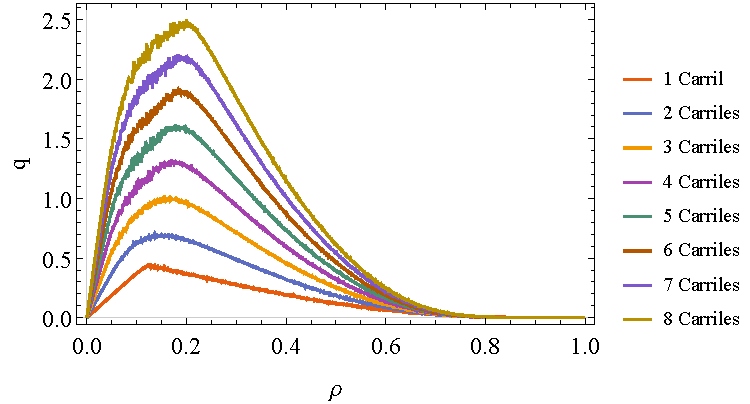
\includegraphics[width=0.8\linewidth]{img/flow_vs_density_multilane}
\caption{Flujo respecto a densidad para diferentes números de carriles.}
\end{figure}

\end{block}

%----------------------------------------------------------------------------------------

\end{column} % End of column 2.2

\end{columns} % End of the split of column 2 - any content after this will now take up 2 columns width


%----------------------------------------------------------------------------------------

\begin{columns}[t,totalwidth=\twocolwid] % Split up the two columns wide column again

\begin{column}{\onecolwid} % The first column within column 2 (column 2.1)

%----------------------------------------------------------------------------------------
%	MATHEMATICAL SECTION
%----------------------------------------------------------------------------------------


%----------------------------------------------------------------------------------------

\end{column} % End of column 2.1

\begin{column}{\onecolwid} % The second column within column 2 (column 2.2)



%----------------------------------------------------------------------------------------

\end{column} % End of column 2.2

\end{columns} % End of the split of column 2

\end{column} % End of the second column

\begin{column}{\sepwid}\end{column} % Empty spacer column

\begin{column}{\onecolwid} % The third column

\begin{block}{Caracterización del tráfico}
Utilizamos la entropía de permutación (EP) para caracterizar el comportamiento caótico del sistema. Se obtiene la EP de la gráfica del gasto, que se genera con un AC de frontera abierta.

\begin{figure}[h!]
\begin{subfigure}{.5\textwidth}
	\centering
	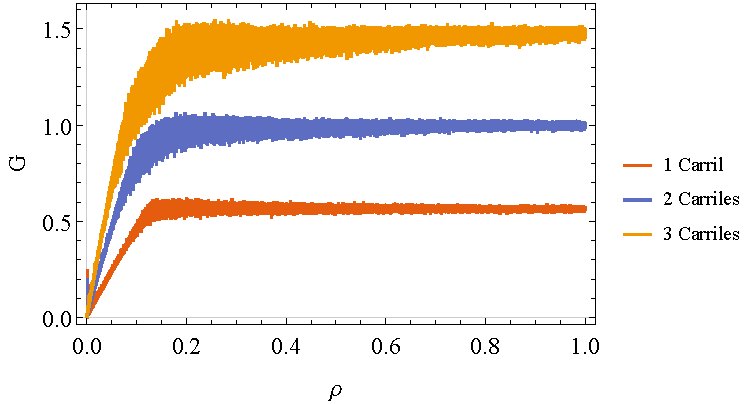
\includegraphics[scale=1.2]{img/discharge_vs_density}
	\caption{Gasto respecto a densidad.}
\end{subfigure}%
\begin{subfigure}{.5\textwidth}
	\centering
	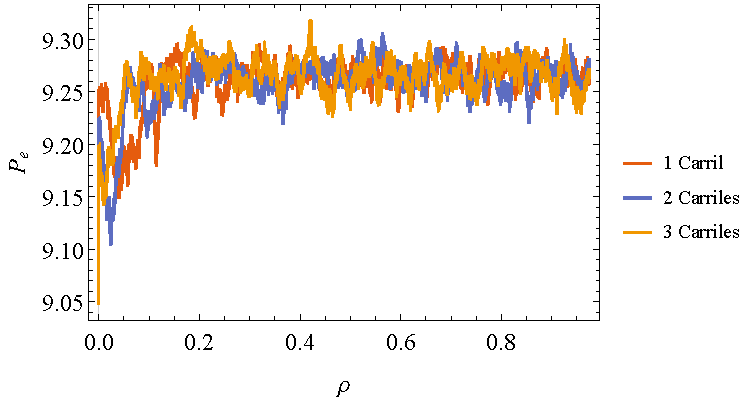
\includegraphics[scale=1.2]{img/pentropy_vs_density}
	\caption{Entropía de permutación de gasto respecto a densidad.}
\end{subfigure}%
\end{figure}

\end{block}	

%----------------------------------------------------------------------------------------
%	CONCLUSION
%----------------------------------------------------------------------------------------

\begin{alertblock}{Conclusiones}

De las simulaciones se observa que para los modelos que se probaron
\begin{enumerate}
\item Los semáforos causan un súbito descenso del flujo, que se caracteriza por su alta variabilidad respecto a su distribución.
\item El número de topes tiene un efecto más leve que el de los semáforos, pero igualmente súbito.
\item Los vehículos autónomos y la adición de más carriles tienen el efecto de aumentar la capacidad de carga del sistema.
\item El comportamiento caótico del tráfico se manifiesta sobre todo después de la transición del flujo.
\end{enumerate}

\end{alertblock}	

%----------------------------------------------------------------------------------------
%	REFERENCES
%----------------------------------------------------------------------------------------




%----------------------------------------------------------------------------------------
%	CONTACT INFORMATION
%----------------------------------------------------------------------------------------

\setbeamercolor{block alerted title}{fg=black,bg=norange} % Change the alert block title colors
\setbeamercolor{block alerted body}{fg=black,bg=white} % Change the alert block body colors

\begin{alertblock}{Información de contacto}

\begin{itemize}
\item Web: \href{https://github.com/CarlosManuelRodr/FreewayAC}{github.com/CarlosManuelRodr/FreewayAC}
\item Email: \href{mailto:fis.carlosmanuel@gmail.com}{fis.carlosmanuel@gmail.com} \href{alej.aguilar.salas@gmail.com}{alej.aguilar.salas@gmail.com}
\end{itemize}

\end{alertblock}

\begin{center}
\begin{tabular}{ccc}

\includegraphics[width=0.4\linewidth]{img/uv_logo} %& \hfill & 
\includegraphics[width=0.4\linewidth]{logo.png}
\end{tabular}
\end{center}

%----------------------------------------------------------------------------------------

\end{column} % End of the third column

\end{columns} % End of all the columns in the poster

\end{frame} % End of the enclosing frame

\end{document}
